\section{Performance testing}

\subsection{Precision of the system}\label{subsec:precisionofsystem}
This experiment will test the precision of the complete system with the
parameters found from simulating the system. The parameters can be found in
\ref{tab:actual_gain_values}

\subsection*{Setup}

The test is performed by fastening a laser pointer on the pan/tilt system. A
board is placed next to the system and two positions where the pointer is on the
board are chosen \ref{fig:systemtestsetup}. The laser pointer is placed 180 cm
from the board. Thus each degree is at around 3 centimetres wide.

\[ \frac{\Pi*2*174}{360} = 3.03687 \]


\begin{figure}[htb] \centering 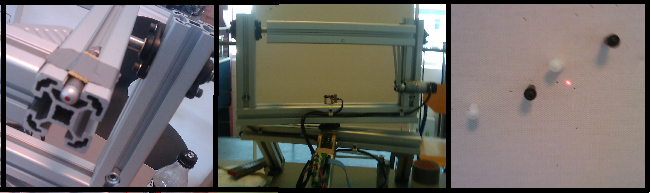
\includegraphics[width=\textwidth,trim=0 0 0
0]{graphics/overallsystemtest.png} %trim=l b r t (can cut off from every side)
	\caption{Setup if the test. From left to right; the mounted laser, the system pointing at the board, laser dot and marks.}
	\label{fig:systemtestsetup}			% figure labels are of the form \label{fig:*}
\end{figure}

The system runs in automode and changes between two setpoints. The positions
are marked and the test ends after ten iterations. 

\subsection*{Results}

At both points the error was less than five centimetres and at most of the time
less than two. This means that the system have an uncertainty between 0.658 and
3.293 degrees. This precision is reached with overshoot.

\[ \frac{2.0}{3.03687} = 0.658 \]

\[ \frac{10.0}{3.03687} = 3.293 \]

\subsection*{Conclusion}

The system itself, have a precision of af third degree.
\[ \frac{360}{160} = 1/3 \]

It is a high precision that have been observed, at times the uncertainty is as
small as the precision of the system. Though it does also show that a higher
precision can be obtained. Overshooting was though occurring in the control.
Additional tuning of the parameters might enhance the performance.

\subsection{Precision of new parameters}\label{sec:precisionofsystem2}

This experiment will test the PID values found in \ref{tab:actual_gain_values}
under best performance.

Here the system will run in automode between two position but only one of the
positions are marked. This is repeated ten times.

\subsection*{Setup}

The setup will be the same as the above \ref{subsec:precisionofsystem}, see
Figure \ref{fig:systemtestsetup}, with the exception that only one point is measured at
the distance 370 centimetres. Thus each degree is 6.458 centimetres wide.

\[ \frac{\Pi*2*370}{360} = 6.458 \]

\subsection*{Results}

In this test the precision of the pan and tilt were recorded to be quite
different. For the tilt was the points precision 7 centimetres were all the
points at the pan was inside two centimetres. Thus the pan/tilt system have
reached precision of respectively 0.310 degrees and 1.083 degrees.


\[ \frac{2}{6.458} = 0.310 \]

\[ \frac{7}{6.458} = 1.083 \]

\subsection*{Conclusion}

The pan has reached a constant precision on par with the system precision
of one third of a centimeter. The tilt part have also become more precise, but
it should be possible to make it even more precise. It could be that because the
tilt is affected by gravity it is harder to control than the pan.


